\documentclass[conference]{IEEEtran}
\IEEEoverridecommandlockouts

\usepackage[utf8]{inputenc}
\usepackage{cite}
\usepackage{amsmath,amssymb,amsfonts}
\usepackage{algorithmic}
\usepackage{graphicx}
\usepackage{textcomp}
\usepackage{xcolor}
\usepackage{bytefield}
\usepackage{url}
\usepackage[whole]{bxcjkjatype}

\def\BibTeX{{\rm B\kern-.05em{\sc i\kern-.025em b}\kern-.08em
    T\kern-.1667em\lower.7ex\hbox{E}\kern-.125emX}}
\begin{document}

\title{Adaptive Source Routing in SRv6 using Programmable SRv6 Functions and eBPF}

\author{\IEEEauthorblockN{Yuzuki Ishiyama (ID:2531008)}
  \IEEEauthorblockA{\textit{Yamaki Laboratory} - \textit{Information and Network Engineering}}
}

\maketitle

\begin{abstract}
  Segment Routing over IPv6 (SRv6) は,現代のネットワークの多様な要件を満たす柔軟なルーティングメカニズムとして注目を集めている.
  しかし,SRv6 には固有の制限がある.ルーティングの決定は送信元で静的に行われるため,パケット送信後に変化するネットワーク状況に適応することが不可能である.
  本研究では,SRv6 Function を用いて適応型ソースルーティングを実現する新しい手法を提案する.
  セグメントリストに経路の分岐条件を直接エンコードすることにより,本手法は追加の制御パケットに頼ることなく,リアルタイムのネットワークメトリックに基づいて動的な経路選択を可能にする.
  我々は,eBPFを用いて Linux ルータ上に本手法を実装し,実験的評価を通じてその実現可能性を示した.
  従来型のプローブベースの手法と比較して,本手法は 43.1\% 高いスループットとより安定したネットワーク品質を示した.
  オーバーヘッドによるスループット低下は 1.04\% であった.
\end{abstract}

\begin{IEEEkeywords}
  service function chaining, segment routing, SRv6, QoS
\end{IEEEkeywords}

\section{Introduction}

インターネットサービスプロバイダ (ISP) は,多様なアプリケーションに対して異なるルーティングポリシーを実装するため,ソースルーティング技術の採用を拡大している\cite{cisco_rakuten_srv6}\cite{softbank_srv6}.
送信元がパケット転送経路を指定するソースルーティングは,従来のホップバイホップ転送と比較して,スケーラビリティと制御性の向上をもたらす.
Segment Routing over IPv6 (SRv6) は,IPv6 拡張ヘッダに経路情報を埋め込むことでソースルーティングを実現するプロトコルである.
他の技術と比較してSRv6 は IPv6 ネットワークへの導入が容易であるため,広く採用されている.

しかしソースルーティングでは,パケット送信時に経路を決定しなければならず,送信後に変化するネットワーク状況に適応できないという根本的な制約がある.
本研究では,この制約を克服するため,SRv6 のセグメントリストに経路の分岐条件を直接エンコードする手法を提案する.
本手法は追加の制御メッセージを必要とせずに,リアルタイムのネットワークメトリックに基づいた動的な経路選択を可能にする.

\section{Background}

\subsection{Source Routing and Potential Issues}

従来のIPルーティングには,複雑なルーティングポリシーの実装が困難であるという課題がある.
これは,各ルータがパケットヘッダの宛先アドレスのみを参照し,自身のルーティングテーブルに基づき独立して次のホップを決定するためである.
その結果,中間ルータはアプリケーションの要件やエンドツーエンドの経路特性を考慮した経路選択を行うことができない.

ソースルーティングは前述の問題を解決し,送信者がパケットがネットワークを通過するべき完全な経路を指定することを可能にする.
このパラダイムは,スケーラビリティと柔軟性を備えたアプリケーション固有のルーティングを提供する.SRv6 は,IPv6 パケットにセグメントルーティングヘッダ (SRH) を追加することによってソースルーティングを実装する\cite{rfc8754}\cite{rfc9256}.
SRH にはセグメントリストが含まれており,これは通過するべきノードを表すセグメント識別子 (SID) のシーケンスである.
ほとんどの場合,SID は IPv6 アドレスである.

しかし,ソースルーティングには根本的な制限がある.
ルーティングの決定は送信元で静的に行われるため,パケット送信後に変化するネットワーク状況に適応することが不可能である.

\subsection{SRv6 Function}

セグメントリストには関数呼び出しを含めることもできる.
この関数はSRv6 Function と呼ばれ,パケットが特定のノードに到達した際に実行される操作を指定する命令である.
各命令は IPv6 アドレスの形式でエンコードされ,Locator,Function,Arguments の3つの部分から構成される.
% 図 \ref{fig:example-of-dividing-an-ipv6-address} は IPv6 アドレスの構造を示している.
Locator は Function が実行されるノードを指し,Function と Arguments はそのノードで実行される操作を指定する.

% show locator, function, and arguments in a bytefield
% | 128 bits                       |
% | 64 bits | 16 bits  | 48 bits   |
% | Locator | Function | Arguments |

% \begin{figure}[htbp]
%   \centering
%   \begin{bytefield}[bitwidth=0.18em]{128}
%     \bitheader{0, 16, 32, 48, 64, 80, 96, 112, 128} \\
%     \bitbox{64}{\small LOC} & \bitbox{16}{\small FUNC} & \bitbox{48}{\small ARG} \\
%   \end{bytefield}
%   \caption{IPv6アドレスの分割例}
%   \label{fig:example-of-dividing-an-ipv6-address}
% \end{figure}

\section{Proposed Method}
% \subsection{Encoding Conditions in SRv6 Function}

基本的なコンセプトは,ネットワークメトリックに基づいた分岐条件とその経路をセグメントリストに含めることである.

セグメントリストに条件付き経路を実装するために,\textit{skip\_if} と \textit{skip} の2つのSRv6 Functionを定義する.
\textit{skip\_if} は帯域などのメトリック条件に基づいて,後続のセグメントを指定した数だけスキップする.
\textit{skip} は単に,後続のセグメントを指定した数だけスキップする
例えば,ある条件 $condition$(例えば,ルータAB間の帯域が閾値を超えた場合,など)が真の場合はルータC,偽の場合はルータBに転送する場合,セグメンリストは $\{ \text{A:\textit{skip\_if}}(1, condition), \text{B:\textit{skip}}(1), \text{C} \}$ となる.

% [Below text] Priority: Low
% メトリック測定におけるノイズを低減するため,メトリックは指数移動平均 (EMA) を用いて平滑化されます.
% EMA は以下の式で計算されます.
% \begin{equation}
%   \text{EMA}_t = \alpha \cdot x_t + (1 - \alpha) \cdot \text{EMA}_{t-1}
% \end{equation}
% ここで,\(x_t\) は現在の測定値,\(\text{EMA}_{t-1}\) は以前の EMA 値,\(\alpha\) は平滑化係数です.

\section{Evaluation Setup}

\begin{figure}[t]
  \centering
  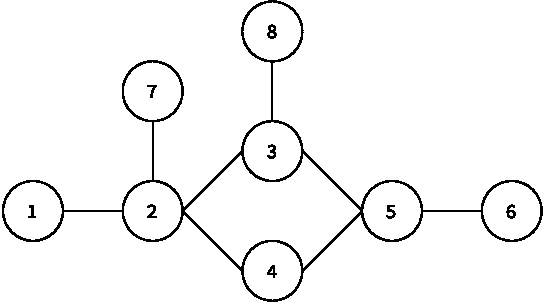
\includegraphics[width=0.7\linewidth]{./figures/topo.pdf}
  \caption{Network Topology}
  \label{fig:network-topology}
\end{figure}


% == OLD START ==
% We evaluated our method using a network topology with multiple potential paths between source and destination nodes. The Linux routers ran our eBPF implementation, and network namespaces, one of the linux features, are used for virtualization, tc for bandwidth/delay control, and iperf3 for traffic generation.
% The proposed method was evaluated using two scenarios:
% \begin{itemize}
%   \item \textbf{Scenario 1}: A single TCP flow that exceeds the threshold, requiring path switching.
%   \item \textbf{Scenario 2}: Two TCP flows competing for bandwidth, with dynamic path selection.
% \end{itemize}
% For comparison, the probe-based approach was also implemented using a separate control packet to probe the network condition.
% == OLD END ==

我々は提案手法について,ネットワーク品質とオーバーヘッドの観点から評価を行った.

ネットワーク品質に関する評価は,図\ref{fig:network-topology} に示すネットワークトポロジーを用いて2つのシナリオを実施した.
各円はルータを示し,ルータ1-2間には遅延 2 ms,ルータ2-3間とルータ2-4間には 1 Gbps の帯域制限を設けた.
1つ目のシナリオでは,ルータ1からルータ6へTCP通信を実行する.
パケットは通常,ルータ2, 3, 5を経由してルータ6に到達するが,ルータ2-3間の帯域が 900 Mbps を超えた場合,超えた分はルータ4を経由してルータ6に到達するように,セグメントリストを設定する.
2つ目のシナリオでは,ルータ1-6間のTCP通信と分岐条件は同一だが,追加でルータ7からルータ8へTCP通信を実行し,追加のTCPフローにより閾値を超えるようにする.
また比較のため,従来型のプローブベースの手法も実装した.これは,ネットワーク状態を調査するために別の制御パケットを使用するものである.

オーバーヘッドの評価は,セグメンリストにSRv6 Functionがある場合とない場合で,TCPスループットを比較することで行った.

\section{Evaluation Results}

% == OLD START ==
% In Scenario 1, the proposed method achieved 43.1\% higher throughput compared to the conventional probe-based approach.
% The performance improvement was attributed to the immediate path switching based on real-time metrics, which avoids TCP congestion control.
% In Scenario 2, our method maintained more stable bandwidth utilization across flows compared to the probe-based approach.
% The implementation overhead was minimal:
% \begin{itemize}
%   \item Protocol size increase: 3.2\%
%   \item Throughput reduction due to eBPF execution: 1.04\%
% \end{itemize}
% == OLD END ==



ネットワーク品質に関する評価結果を示す.
シナリオ1では,提案手法は従来手法と比較して 43.1\% 高いスループットを達成した(図\ref{fig:scenario-1}).
またシナリオ2では,提案手法は従来手法と比較して,より安定したスループットを達成した(図\ref{fig:scenario-2}).
ただし,20秒から40秒がルータ7-8間でTCP通信を実行した区間である.

オーバーヘッドに関する評価では,セグメンリストにSRv6 Functionを含む場合,含まない場合と比較してTCPスループットは1.04\%低下した.

% == OLD START ==
% We proposed and implemented an adaptive source routing method using SRv6 Functions that enables dynamic path selection based on real-time network metrics.
% By encoding conditional logic directly into the Segment List, each router can make forwarding decisions based on the current network conditions.
% Experimental results demonstrated higher throughput and more stable performance compared to a conventional probe-based approach with minimal overhead.
% Future work includes supporting additional metrics and more complex conditions.
% == OLD END ==

\section{Discussion}

提案手法は,SRv6 Function を活用し,セグメントリスト内に経路の条件分岐を直接組み込むことで,適応型ソースルーティングを実現する新しい手法を提示した.
評価実験の結果,本手法は従来のプローブベースの手法と比較して,ネットワークスループットと安定性の両面で顕著な改善を示した.
特に,シナリオ1で見られた43.1\%のスループット向上は,提案手法がネットワーク状態の変化をリアルタイムで検知し,即座に経路を最適化できる能力によるものである.これにより,従来手法に見られるような,状態検知の遅延や,それに起因するTCP輻輳制御メカニズムの非効率な動作を回避することが可能となる.
同様に,シナリオ2におけるスループットの安定性向上も,この迅速な適応能力が寄与していると考えられる.
実装面では,eBPFを用いた本手法の実行オーバーヘッドはスループット低下1.04\%と非常に小さく,プロトコルヘッダサイズの増加も限定的であった.
本研究では主に帯域幅を判断基準としたが,将来的には遅延,ジッター,パケットロス率など,より多様なネットワークメトリックを組み合わせた複雑な条件分岐ロジックの実現も期待される.

\begin{figure}[t]
  \centering
  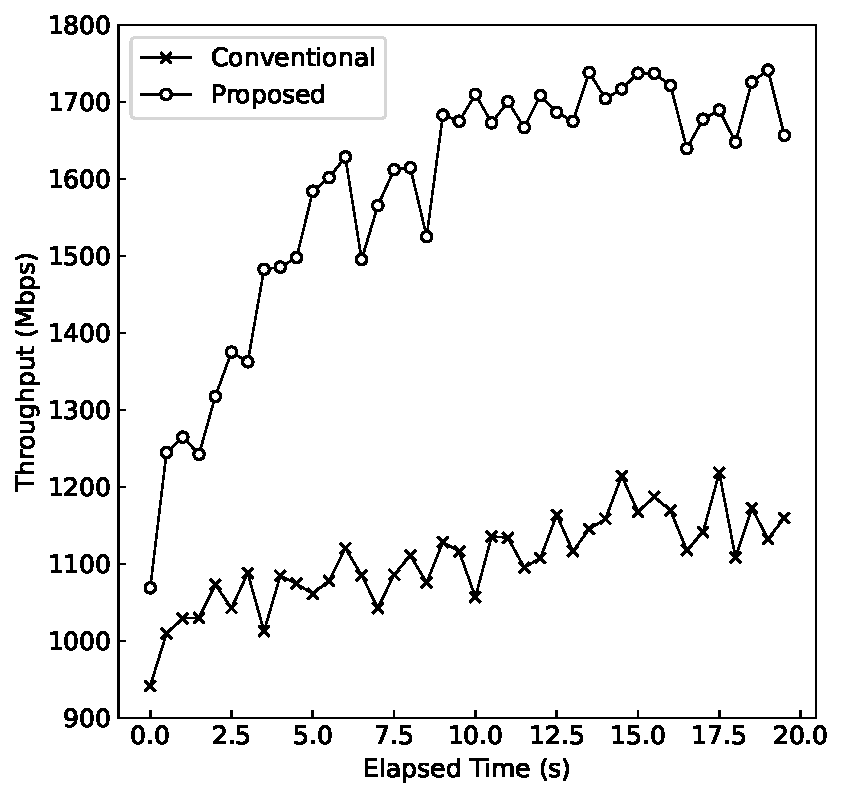
\includegraphics[width=0.7\linewidth]{./figures/scenario-1.pdf}
  \caption{Scenario 1: TCP Throughput}
  \label{fig:scenario-1}
\end{figure}

\begin{figure}[t]
  \centering
  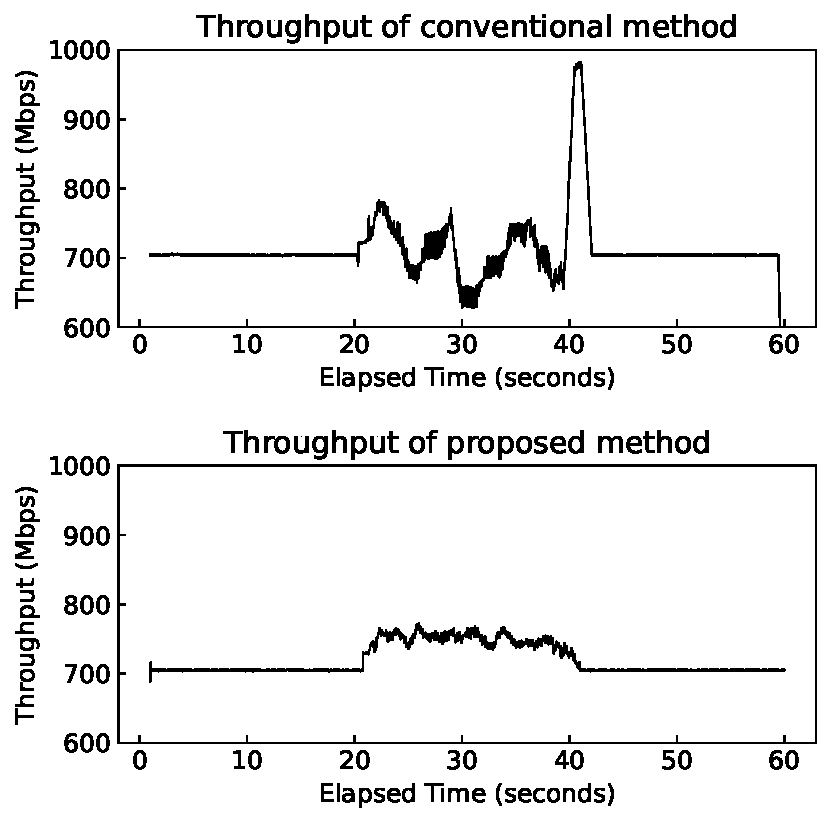
\includegraphics[width=0.7\linewidth]{./figures/scenario-2.pdf}
  \caption{Scenario 2: TCP Throughput}
  \label{fig:scenario-2}
\end{figure}

\section{Conclusion}

本研究では,SRv6 Function を用いて適応型ソースルーティングを実現する新しい手法を提案した.
本手法は,セグメントリストに経路の分岐条件を直接エンコードすることにより,追加の制御パケットに頼ることなく,リアルタイムのネットワークメトリックに基づいて動的な経路選択を可能にする.
eBPFを用いて Linux ルータ上に本手法を実装し,実験的評価を通じてその実現可能性を示した.
従来型のプローブベースの手法と比較して,本手法は高いスループットとより安定したネットワーク性能を示した.
実装のオーバーヘッドは最小限であった.
今後の課題としては,追加のメトリックやより複雑な条件のサポートが挙げられる.

\bibliographystyle{IEEEtran}
\bibliography{refs}

\end{document}
